Consider the annual rates of return (including dividends) on the Dow-Jones
industrial average for the years 1996--2005. These data, multiplied by 100, are
$\begin{NiceArray}{rrrrrrrrr}
    -0.6 & 3.1 & 25.3 & -16.8 & -7.1 & -6.2 & 25.2 & 22.6 & 26.0
\end{NiceArray}$.
\newline
% -0.6 3.1 25.3 -16.8 -7.1 -6.2 25.2 22.6 26.0
Use these 10 observations to complete the following.
\begin{enumerate}[label= (\alph*)]
    \item Construct a Q-Q plot. Do the data seem to be normally distributed? Explain.
    \begin{figure}[H]
        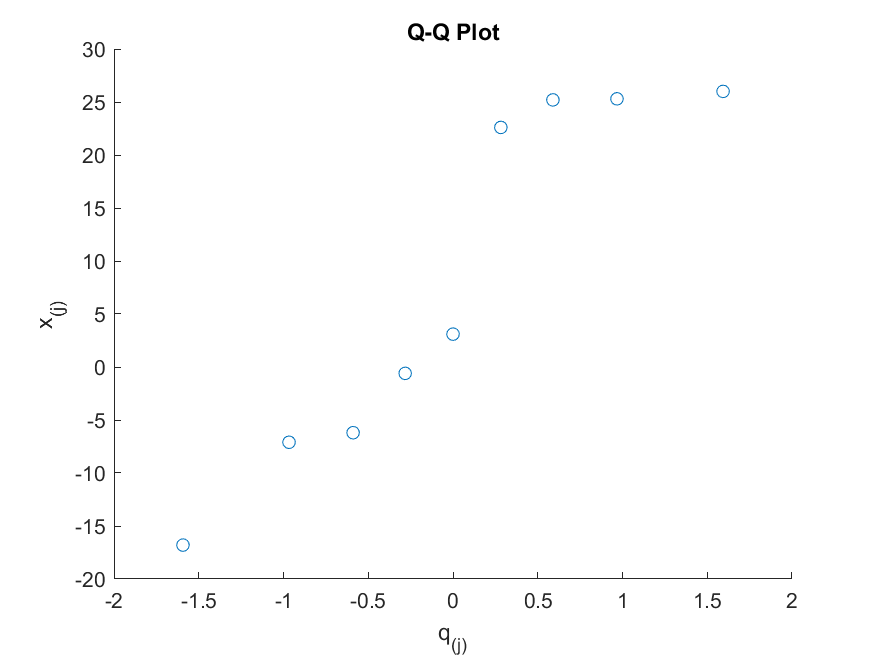
\includegraphics[scale=0.8]{./matlab/chapter-4/sol4.23a.png}
    \end{figure}
    \item Carry out a test of normality based on the correlation coefficient $r_{Q}$. [See (4--31).]
    Let the significance level be $\alpha = .10$.
    \begin{equation*}
        \begin{aligned}
            H_{0}: & \text{\ The data is normally distributed.} \\
            H_{\alpha}: & \text{\ The data is NOT normally distributed.}
        \end{aligned}
    \end{equation*}
    The $r_{Q}$ value is 0.9351. From table 4.2, using $\alpha = 0.10$ and sample size $n = 10$, the critical point is 0.9351. We only have 9 observations, so the citical value is slightly less, so $r_{Q} \geq 0.9351$, so we'd conclude the data is normal. It's right on the border though.
    \newline
    \hspace{0.5in} Going the extra mile, using the Filliben paper from Reference 5 in Chaper 4, \textit{The Probability Plot Test for Correlation coefficient Test for Normality} we can simulate values just like those in Table 4.2, but for a sample size of 9. The simulation invlolves generating 9 points from a standard normal and sorting the 9 values. The probability levels are computed and standard normal quantiles are computed (just like in Example 4.9). The correlation coefficient is computed using the data and the quantiles. The correlation coefficient is then saved. This was performed $N = 10^{6} = 1\text{M}$ times (1M samples). In the Filliben paper, there were $N = 10^{5} = 100\text{K}$ samples genereated. The 1M values were used to create quantile at the 0.10-level. The simulated value was 0.9295314. This is smaller than the $r_{Q}$ value of 0.9351. Based on the simulated value we would conclude $H_{0}$, that the data is normally distributed. The histogram of the simulated values is below. In the plot 10\% of the data lies below the red dashed vertical line at the value 9295314.
    \begin{figure}[H]
        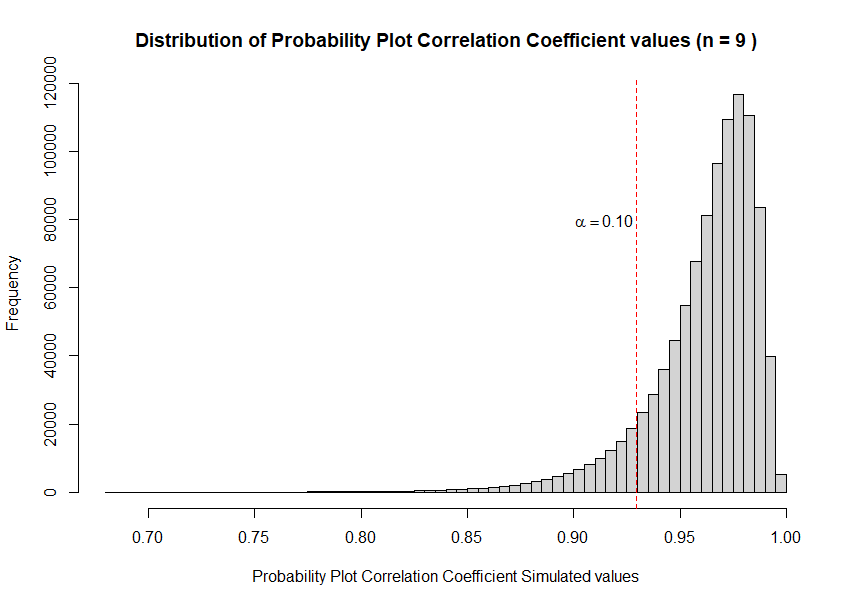
\includegraphics[scale=0.5]{./r/chapter-4/sol4.23b.png}
    \end{figure}
\end{enumerate}